\documentclass[11pt]{beamer}
\usepackage[utf8]{inputenc}
\usepackage[spanish]{babel}
%\usepackage{amsmath}
%\usepackage{amsfonts}
%\usepackage{amssymb}
%\usepackage{graphicx}
\usepackage{subfigure} % subfiguras
\usepackage{ragged2e}
%\usepackage{hyperref}
\usepackage{float}
\usepackage{url}
\usepackage{listings}
\usepackage{xcolor}
\usepackage{algorithm,algorithmic}


\definecolor{codegreen}{rgb}{0,0.6,0}
\definecolor{codegray}{rgb}{0.5,0.5,0.5}
\definecolor{codepurple}{rgb}{0.58,0,0.82}
\definecolor{backcolour}{rgb}{0.95,0.95,0.92}

\lstdefinestyle{style_code}{
    backgroundcolor=\color{backcolour},   
    commentstyle=\color{codegreen},
    keywordstyle=\color{magenta},
    numberstyle=\tiny\color{codegray},
    stringstyle=\color{codepurple},
    basicstyle=\ttfamily\footnotesize,
    breakatwhitespace=false,         
    breaklines=true,                 
    captionpos=b,                    
    keepspaces=true,                 
    numbers=left,                    
    numbersep=5pt,                  
    showspaces=false,                
    showstringspaces=false,
    showtabs=false,                  
    tabsize=2
}

\lstset{style=style_code}

\usetheme{Madrid}

%\usepackage{natbib}
\usepackage{bibentry}
\usepackage{graphicx} % Allows including images
\usepackage{booktabs} % Allows the use of \toprule, 

\setbeamertemplate{bibliography item}{\insertbiblabel}

\newcommand{\celda}[1]{
	\begin{minipage}{2.5cm}
		\vspace{5mm}
		#1
		\vspace{5mm}
	\end{minipage}
}

\author[Abarca, Apari, Suca, Vargas] % (optional)
{J.~P.~Abarca\inst{1} \and C.~T.~Apari\inst{1} \and C.~A.~Suca\inst{1} \and A.~Vargas\inst{1}  }
\title[Practica1]{Práctica 1}
\date{ 26 de Junio del 2021} 
%\date{\currenttime}
\subtitle{Algoritmos de Ordenamiento}
\logo{
\includegraphics[scale=0.16]{unsa.png}}
\institute[UNSA]{
	\inst{1}
		Universidad Nacionan del San Agustin. Facultad de Producción y Servicios. \\Escuela Profesional de Ciencias de la Computación\\
		Maestría en Ciencias de la Computación \\ Docente: Mg. Vicente Machaca \\
		\vspace{2mm}
}

\AtBeginSection[]
{
	\begin{frame}<beamer>{Contenido}
		\tableofcontents[currentsection,currentsubsection]
	\end{frame}
}

\begin{document}

    
	
	\begin{frame}
		\maketitle
	\end{frame}

	\begin{frame}{Contenido}
		\tableofcontents
	\end{frame}

	\section{Resumen}
		\begin{frame}{Resumen}
			\justifying
			\begin{itemize}
			    \item Se realizó la implementación de algoritmos de ordenamiento y la medición de su respectivo tiempo de ejecución graficados.
			    \item La implementación de los algoritmos se realizó en dos lenguajes de programación: C++ y Python, para realizar la medición se crearon archivos con elementos desordenados, cada algoritmo genera un archivo *.txt resultante con la cantidad de datos y el tiempo de ejecución, finalmente estos resultados se graficaron para mostrar las diferencias entre lenguaje de programación y algoritmo.
			\end{itemize}
		\end{frame}
	
	\section{Preparación de Datos}
		\begin{frame}{Preparación de Datos}
			\justifying
			\begin{itemize}
			    \item Se generaron 21 archivos con números generados aleatoriamente.
			    \item Cada archivo contiene 100, 500, 1000, 2000, 3000, ..., 10000, 20000, 30000, ..., 1000000 números con la denominación ejemplo\textunderscore $<$número$>$
			\end{itemize}
			
			\begin{figure}[H]
				\centering
				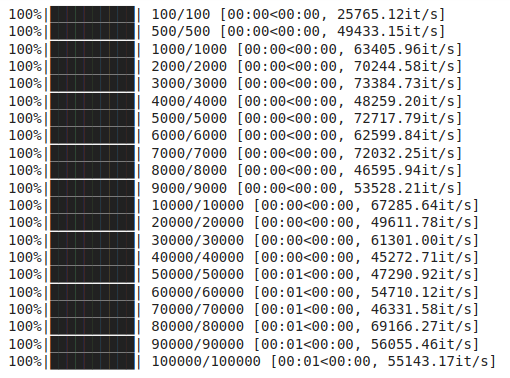
\includegraphics[scale=0.40]{img/1_preparacion_datos.png}
				\caption{Archivos generados}
				\label{fig: prep_datos_fig1}
			\end{figure}
		\end{frame}
		
		\begin{frame}{Preparación de Datos - Codigo (parte 1)} 
			\lstinputlisting[language=Python, firstline=1, lastline=8, caption=Generación de Números(parte 1)]{code/generatedFiles.py}
		\end{frame}
		\begin{frame}{Preparación de Datos - Codigo (parte 2)} 
			\lstinputlisting[language=Python, firstline=9, lastline=19, caption=Generación de Números(parte 2)]{code/generatedFiles.py}
		\end{frame}
	
	\section{Implementación de algoritmos}
		\begin{frame}{Desarrollo}
			\justifying
			\begin{itemize}
			    \item Para la implementación de cada algoritmo se tomaron los archivos generados en el primer punto.
			    \item Cada algoritmo implementado ordenara los números generados por cada archivo.
			    \item Cada vez que calcule a cada archivo este generará un nuevo archivo *.txt mostrando la cantidad de números revisado con el tiempo de ejecución.
			\end{itemize}
		\end{frame}
		
		\subsection{Bubble Sort}
		\begin{frame}{BubbleSort - Definición}
		    \begin{itemize}
		         \item El procedimiento de ejecución comienza con un arreglo de números enteros distribuidos de forma aleatoria, los cuales deben ser ordenados con una búsqueda secuencial sobre los elementos ya procesados, esto consiste en recorrer una y otra vez los elementos del arreglo que ya fueron ordenados, encontrar una posicion especifica e intercambiar con el elemento seleccinoado.
		    \end{itemize}
		    \begin{algorithm}[H]
                \begin{algorithmic}[1]
                    \FOR{$i \gets 1$ to $N$}
                        \FOR{$j \gets i+1$ to $N$}
                            \IF{$A[j] < A[i]$}
                                \STATE $temp \gets A[i]$
                                \STATE $A[i] \gets A[j];$ 
                                \STATE $A[j] \gets temp;$
                            \ENDIF    
                        \ENDFOR
                    \ENDFOR
                \end{algorithmic}
                \caption{BUBBLE-SORT(A)}
                \label{alg:bubble-sort}
            \end{algorithm}
		\end{frame}
		\begin{frame}{BubbleSort - Análisis}
            \begin{itemize}
                \item La complejidad computacional del algoritmo es $O(n^{2})$, en el peor y mejor caso. Siendo \textit{n} la cantidad de elementos a ordenar.
                \item La comparacion del tiempo de ejecucion del algoritmo Bubble Sort en los lenguajes C++ y Python, teniendo como mas optimo al C++.
            \end{itemize}
            \begin{figure}[H]
				\centering
				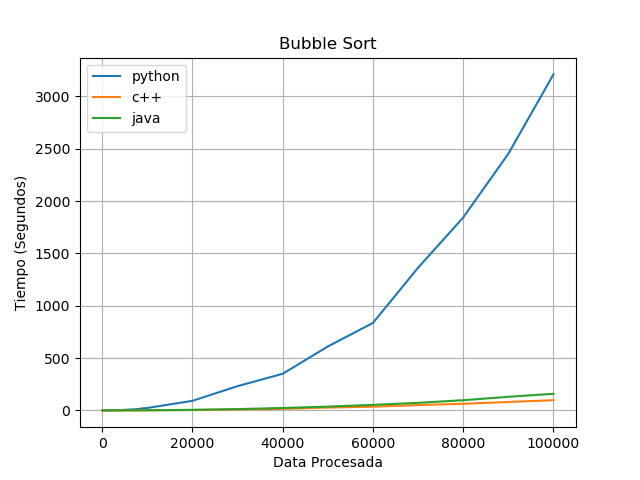
\includegraphics[scale=0.40]{img/bubble_sort_grafica.png}
				\caption{Bubble Sort - Tiempo de Ejecución}
				\label{fig:bubble_sort_grafica}
			\end{figure}
		\end{frame}
		
		\subsection{Counting Sort}
		\begin{frame}{CountingSort - Definición}
		     \begin{itemize}
		         \item Permite ordenar números sin necesidad de realizar comparaciones, usando un contador para almacenar los valores repetidos del arreglo.
		     \end{itemize}
		     \begin{algorithm}[H]
                \begin{algorithmic}[1]
                    \FOR{$i \gets 0$ to $K$}
                        \STATE $C[i] \gets 0$
                    \ENDFOR
                    \FOR{$j \gets 1$ to $length[A]$}
                        \STATE $C[A[j]] \gets C[A[j]] + 1$
                    \ENDFOR
                    \FOR{$i \gets 1$ to $k$}
                        \STATE $C[i] \gets C[i] + C[i - 1]$
                    \ENDFOR
                    \FOR{$j \gets length[A]$ to $1$}
                        \STATE $B[C[A[j]]] \gets A[j]$
                        \STATE $C[A[j]] \gets C[A[j]]-1$
                    \ENDFOR
                \end{algorithmic}
                \caption{COUNTING-SORT(A,B,k)}
                \label{alg:counting-sort}
            \end{algorithm}
		\end{frame}
		\begin{frame}{CountingSort - Funcionamiento}
		     \begin{figure}[H]
				\centering
				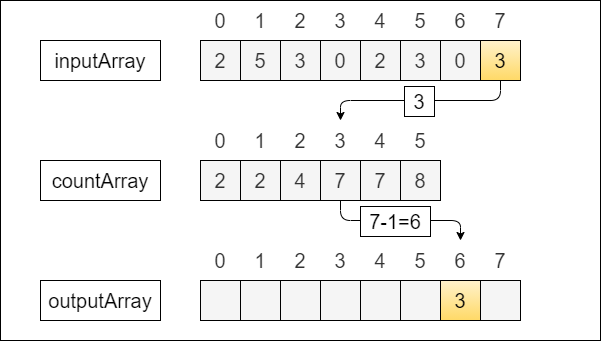
\includegraphics[scale=0.40]{img/countingsort.png}
				\caption{Counting Sort}
				\label{fig:counting_sort_img1}
			\end{figure}
		\end{frame}
		\begin{frame}{CountingSort - Análisis}
            \begin{itemize}
                \item La complejidad computacional del algoritmo es $O(n+k)$, en el peor y mejor caso.
            \end{itemize}
            \begin{figure}[H]
                \centering
                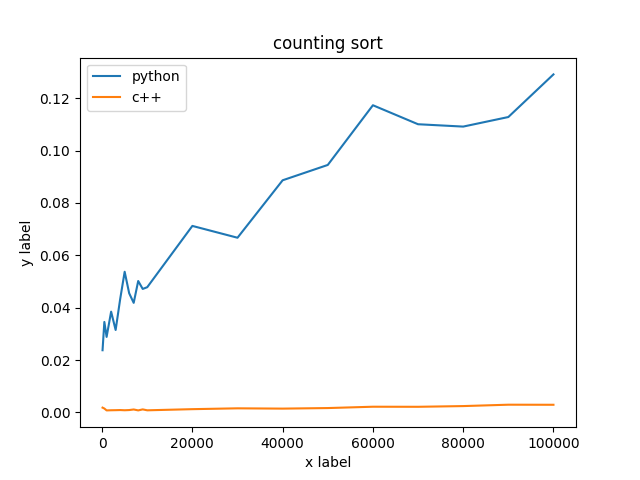
\includegraphics[scale=0.5]{img/counting_diagram.png}
                \caption{CountingSort - Tiempo de Ejecución}
                \label{fig:counting_diagram}
            \end{figure}
            
		\end{frame}
		\subsection{Heap Sort}
		    \begin{frame}{HeapSort - Definición}
    		     \begin{itemize}
    		         \item Esta estructura basada en un \'{a}rbol binario mantiene una propiedad o invariante de que en cada nivel cualquier nodo sea siempre mayor a sus hijos $A[Parent(i)] \geq A[i]$, como se observa en la figura \ref{fig:heap_trace}.
    		         
    		        \begin{figure}[H]
    		            \centering	 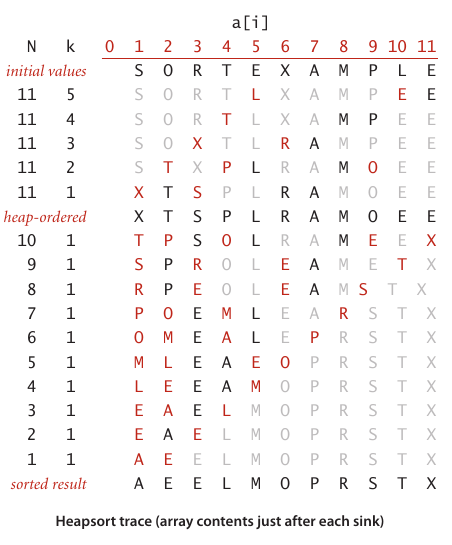
\includegraphics[scale=0.40]{img/heapsort_trace.png}
                        \caption{Aplicaci\'{o}n del algoritmo Heapsort: Construcción y SortDown \cite{Algorithms}}
                        \label{fig:heap_trace}
                    \end{figure}
    		     \end{itemize}
    		\end{frame}
    		\begin{frame}{HeapSort - Definición}
    		     \begin{itemize}
    		         \item El primer proceso es Build-Max-Heap, el principal objetivo es hacer cumplir la invariante, el cual es que todo nodo padre sea mayor a sus nodos hijo, en caso de no serlo se producir\'{a} el intercambio y recursivamente se ayudar\'{a} de la funci\'{o}n Max-Heapify haciendo la propagaci\'{o}n hacia abajo.
    		         
    		        \begin{algorithm}[H]
                        \begin{algorithmic}[1]
                            \STATE $heap-size[A] \leftarrow length[A]$
                            \FOR{$i \leftarrow \lfloor length[A]/2 \rfloor$ to $1$}
                                \STATE $Max-Heapify(A,i)$
                            \ENDFOR
                        \end{algorithmic}
                        \caption{Build-Max-Heap(A)}
                        \label{alg:build-max-heap}
                    \end{algorithm}
    		     \end{itemize}
    		\end{frame}
    		\begin{frame}{HeapSort - Definición}
    		     \begin{itemize}
    		         \item El segundo proceso, es el SortDown aplicando Max-Heapify quien se encarga de hacer cumplir la invariante.
    		         
    		        \begin{algorithm}[H]
                        \begin{algorithmic}[1]
                            \STATE $l \leftarrow LEFT(i)$
                            \STATE $r \leftarrow RIGHT(i)$
                            \IF{ $l \leq heap-size[A]  \AND  A[l] > A[i]$}
                                \STATE $largest \leftarrow l$
                            \ELSE
                                \STATE $largest \leftarrow i$
                            \ENDIF
                            \IF{ $r \leq heap-size[A] and A[r] > A[largest]$}
                                \STATE $largest \leftarrow r$
                            \ENDIF
                            \IF{ $largest \neq i$}
                                \STATE $exchange A[i] \leftrightarrow A[largest]$
                                \STATE $Max-Heapify(A, largest)$
                            \ENDIF
                        \end{algorithmic}
                        \caption{Max-Heapify(A,i)}
                        \label{alg:max-heapify}
                    \end{algorithm}
    		     \end{itemize}
    		\end{frame}
    		\begin{frame}{HeapSort - Definición}
    		     \begin{itemize}
    		         \item El completo algoritmo de heapsort es dado en el seudoc\'{o}digo \ref{alg:heapsort}
    		         
    		        \begin{algorithm}[H]
                        \begin{algorithmic}[1]
                            \STATE $BUILD-MAX-HEAP(A)$
                            \FOR{$i \leftarrow length[A]$ downto $2$}
                                \STATE exchange $A[1] \leftrightarrow A[i]$
                                \STATE $heap-size[A] \leftarrow heapsize[A]-1$
                                \STATE $MAX-HEAPIFY(A,1)$
                            \ENDFOR
                        \end{algorithmic}
                        \caption{Heapsort(A)}
                        \label{alg:heapsort}
                    \end{algorithm}
    		     \end{itemize}
    		\end{frame}
    		\begin{frame}{HeapSort - Análisis}
    		     \begin{itemize}
    		         \item El procedimiento de Heapsort toma un tiempo de O(nlgn).
    		         
                     \item El Build-Max-Heap toma un tiempo lineal O(n), la altura de los mont\'{i}culos, multiplicado por el n\'{u}mero de nodos dados en un nivel particular, esto sumado por cada nivel de la construcción en el \'{a}rbol, da un orden lineal O(n).
                            
                     \item En cuanto al proceso de SortDown se realizar n-1 llamadas de Max-Heapify interno el cual por si solo tiene un coste de O(lgn), en este caso Max-Heapify toma un coste de acuerdo a la altura del montículo. Es así que el coste total de el proceso de SortDown es O(nlgn) y es el coste del proceso de Heapsort.
    		     \end{itemize}
    		\end{frame}
    		\begin{frame}{HeapSort - Análisis}
    		     \begin{itemize}
    		         \item En la siguiente gráfica \ref{fig:heapsort_diagram} se muestra la comparación de los tiempo tomados para el heapsort en 3 lenguajes Python, Java, y C++, donde se observa el crecimiento casi lineal del tiempo tomado por Python conforme la carga de datos crece.
                            
                    \begin{figure}[H]
                        \centering 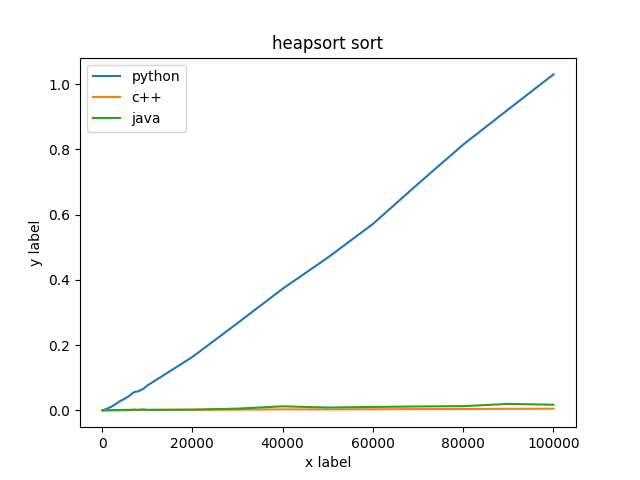
\includegraphics[scale=0.4]{img/heapsort_diagram.png}
                        \caption{Heapsort - Tiempo de Ejecución}
                        \label{fig:heapsort_diagram}
                    \end{figure}
    		     \end{itemize}
    		\end{frame}
		%%%% INSERTION SORT
		\subsection{Insertion Sort}
		
		    \begin{frame}{Insertion Sort - Definición}
    		    \begin{algorithm}[H]
                    \begin{algorithmic}[1]
                        \FOR{$i \gets 1$ to $N$}
                            \STATE $key \gets A[i]$
                            \STATE $j \gets i-1$
                            \WHILE{$j>=0$ and $A[j] > key$}
                                \STATE $A[j + 1] \gets A[j]$ 
                                \STATE $j \gets j - 1$
                            \ENDWHILE
                            \STATE $A[j + 1] \gets key$
                        \ENDFOR
                    \end{algorithmic}
                    \caption{INSERTION-SORT(A)}
                    \label{alg:insertion-sort}
                \end{algorithm}
    		\end{frame}
    		
    		\begin{frame}{Insertion Sort - Análisis}
    		     \begin{itemize}
    		         \item Similar a la manera de ordenar una baraja de un juego de naipes en las manos. El array es virtualmente dividido en una parte ordenada y otra desordenada, los valores de la parte desordenada es elegida y ubicada en la posición correcta en la parte ordenada. 
    		         \item El algoritmo tiene un costo de $O(n^2)$ \cite{CLRS2009}
    		         
    		         \begin{figure}[H]
        				\centering
        				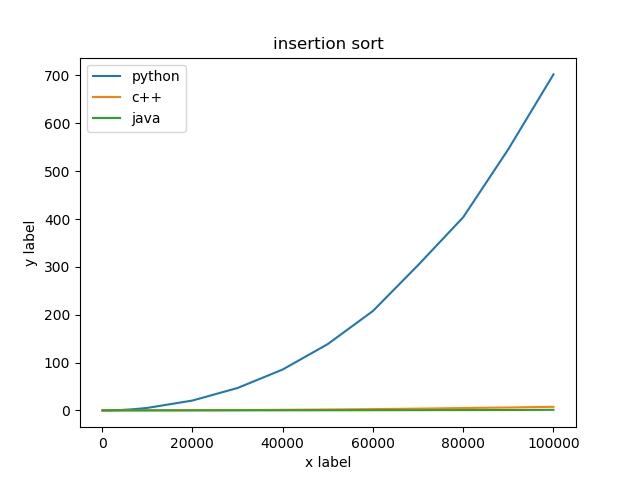
\includegraphics[scale=0.35]{img/insertion_diagram.png}
        				\caption{Tiempo de Ejecución Insertion Sort}
        				\label{fig: insertion_sort_fig1}
        			\end{figure}
    		         
    		     \end{itemize}
    		    
    		\end{frame}
		
		\subsection{Merge Sort}
		\begin{frame}{MergeSort - Definición}
		     
	        \begin{itemize}
	            \item Se basa en la técnica divide y vencerás.
	            \item Dividir el arreglo no ordenado en dos subarreglos(la mitad del arreglo principal), mezcla las sublistas hasta completar el arreglo principal.
	            \end{itemize}
    		            
		      \begin{algorithm}[H]
                \begin{algorithmic}[1]
                        \IF {$r > p$} 
                            \STATE $m \gets p + (r-p)/2$ 
                            \STATE CALL mergeSort(A,p,m)
                            \STATE CALL mergeSort(A,m+1,r)
                            \STATE CALL merge(A,p,m,r)
                        \ENDIF
                \end{algorithmic}
                \caption{MERGE-SORT(A,p,r)}
                \label{alg:merge-sort}
            \end{algorithm}
		\end{frame}
		\begin{frame}{MergeSort - Definición}
		     \begin{algorithm}[H]
                \begin{algorithmic}[1]
                    \STATE $n1 \gets q-p+1$
                    \STATE $n2 \gets r-q$
                    \STATE create arrays L[1..n1+1] and R[1..n2+1]
                    \FOR{$i \gets 1$ to $n1$}
                        \STATE $L[i] \gets A[p+i-1]$
                    \ENDFOR
                    \FOR{$j \gets 1$ to $n2$}
                        \STATE $R[j] \gets A[q+j]$
                    \ENDFOR
                    \STATE $i \gets 1$
                    \STATE $j \gets 1$
                    \STATE $k \gets l$
                    \WHILE{$i < n1$ and $ j < n2$}
                        \IF {$L[i] <= R[j]$} 
                            \STATE $A[k] \gets L[i]$ 
                            \STATE $i \gets i + 1$ 
                        \ELSE
                            \STATE $A[k] \gets R[j]$ 
                            \STATE $j \gets j + 1$
                        \ENDIF
                        \STATE $k = k + 1;$
                    \ENDWHILE
                    \WHILE{$i < n1$}
                        \STATE $A[k] = L[i]$
                        \STATE $i = i + 1;$
                        \STATE $k = k + 1;$
                    \ENDWHILE
                    \WHILE{$j < n2$}
                        \STATE $A[k] = R[j]$
                        \STATE $j = j + 1;$
                        \STATE $k = k + 1;$
                    \ENDWHILE
                \end{algorithmic}
                \caption{MERGE(A,p,q,r)}
                \label{alg:merge}
            \end{algorithm}
		\end{frame}
		\begin{frame}{MergeSort - Funcionamiento}
		     \begin{figure}[H]
				\centering
				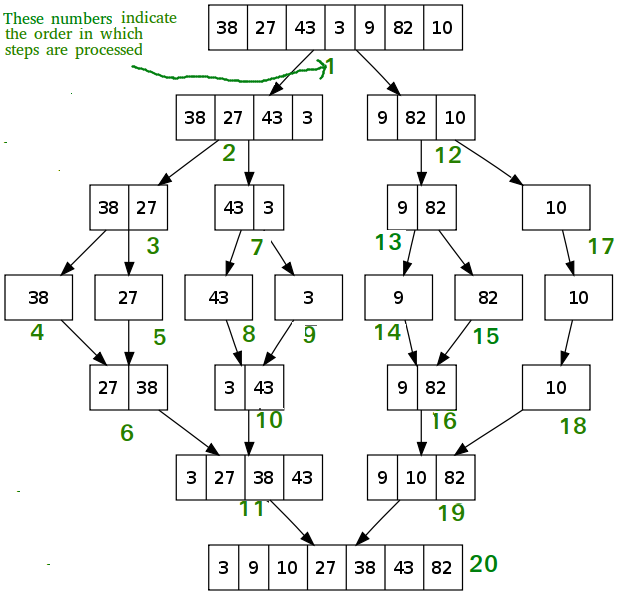
\includegraphics[scale=0.30]{img/mergesort.png}
				\caption{Merge Sort}
				\label{fig:merge_sort_img1}
			\end{figure}
		\end{frame}
		\begin{frame}{MergeSort - Análisis}
            \begin{itemize}
                \item La complejidad del algoritmo es $O(n log n)$.
                \item No trabaja in situ, es decir no cambia directamente el valor en el arreglo.
                \item Para mezclar dos subarreglos, deben estar ordenados.
                \item Requiere un espacio auxiliar $O(n)$, en comparación con Heapsort que requiere un espacio de $O(1)$
            \end{itemize}
            \begin{figure}[H]
                \centering
                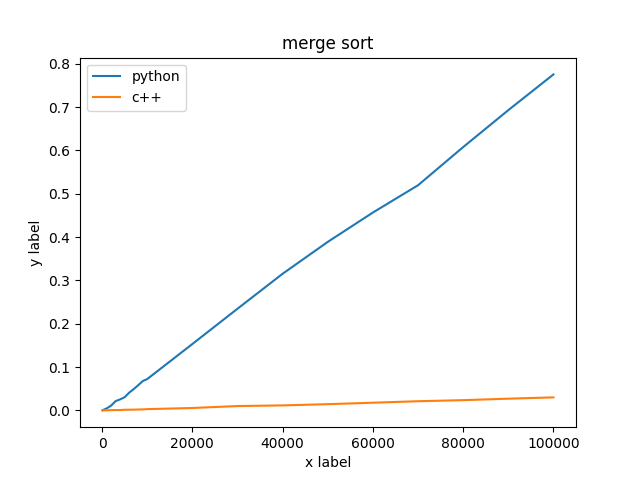
\includegraphics[scale=0.4]{img/merge_diagram.png}
                \caption{MergeSort - Tiempo de Ejecución}
                \label{fig:merge_diagram}
            \end{figure}
            
		\end{frame}
		\subsection{Quick Sort}
		    \begin{frame}{QuickSort Definición}
		        \begin{itemize}
		            \item El algoritmo de Quicksort fue inventado por el autor C.A.R. Hoare en 1960, este algoritmo es bastante eficiente y es garantizado el ordenamiento, en el peor caso con un orden de $O(n^2)$ y en el caso promedio $O(n\log(n))$, el ordenamiento es en lugar, solo requiere una pequeña pila adicional.
		            
		            En el siguiente seudoc\'{o}digo \ref{alg:quicksort} se da la implementaci\'{o}n del algoritmo quicksort.
    		        
    		        \begin{algorithm}[H]
                        \begin{algorithmic}[1]
                            \IF{$p<r$}
                                \STATE $q \leftarrow Partition(A,p,r)$
                                \STATE $QUICKSORT(A,p,q-1)$
                                \STATE $QUICKSORT(A,q+1,r)$
                            \ENDIF
                        \end{algorithmic}
                        \caption{QUICKSORT(A,p,r)}
                        \label{alg:quicksort}
                    \end{algorithm}
                    
                    
		        \end{itemize}
		    \end{frame}
		    \begin{frame}{QuickSort Definición}
		        \begin{itemize}
		            \item El factor mas importante en el algoritmo de Quicksort es el proceso de partici\'{o}n , dado por el siguiente seudoc\'{o}digo \ref{alg:quick_partition}
		            
		            \begin{algorithm}[H]
                        \begin{algorithmic}[1]
                            \STATE $x \leftarrow A[r]$
                            \STATE $i \leftarrow p-1$
                            \FOR{$j \leftarrow p$ to $r-1$}
                                \IF{$A[j] \leq x$}
                                    \STATE $i \leftarrow i+1$
                                    \STATE $A[i] \leftrightarrow A[j]$
                                \ENDIF
                            \ENDFOR
                            \STATE exchange $A[i+1] \leftrightarrow A[r]$
                            \STATE return i+1
                        \end{algorithmic}
                        \caption{PARTITION(A,p,r)}
                        \label{alg:quick_partition}
                    \end{algorithm}
		        \end{itemize}
		    \end{frame}
		    
		    \begin{frame}{QuickSort Definición}
		        \begin{itemize}
		            \item El proceso de partici\'{o}n implica tomar el \'{u}ltimo elemento del array como pivote $x = A[r]$ el cual ser\'{a} el elemento que divida y genere los dos subarrays, en la inicializaci\'{o}n de los iteradores $i$ y $j$ se generan 4 regiones, como se observa en la figura \ref{fig:quicksort_regions}
                    
                    \begin{figure}[H]
                        \centering
                        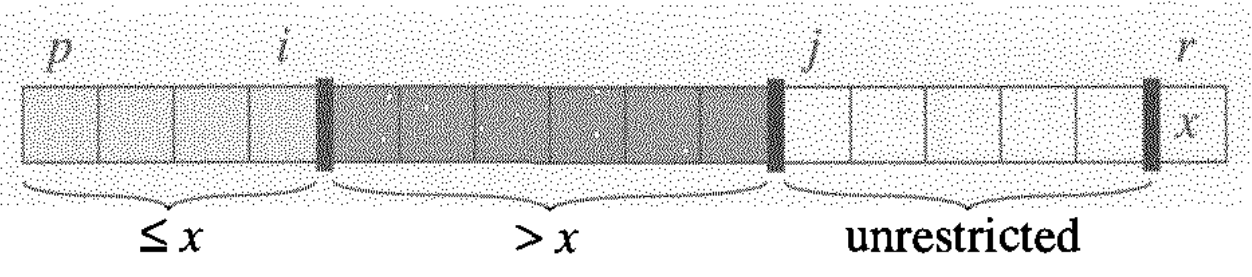
\includegraphics[scale=0.20]{img/quicksort_regions.png}
                		\caption{Regiones en el Partition}
                		\label{fig:quicksort_regions}
                	\end{figure}
		        \end{itemize}
		    \end{frame}
		    
		    \begin{frame}{Quickort Análisis}
		        \begin{itemize}
		            \item \textbf{Pero Caso} Resolviendo al recurrencia el tiempo tomado para el peor caso se produce un tiempo de $T(n) = O(n^2)$, es as\'{i} que es muy similar al caso del insertion sort, y esto ocurre cuando los elmentos de ingreso ya est\'{a}n completamente ordenados, en este caso insertion sort gana con un orden de $O(n)$.
                    \item \textbf{Mejor Caso} Si se diera el caso de que los subarrays sean de tama\~{n}o no m\'{a}s de $n/2$, la recurrencia para el tiempo de ejecuci\'{o}n es: $T(n) = 2T(n/2) + \Theta(n)$ esta recurrencia tiene la soluci\'{o}n de $T(n) = O(nlgn)$.
                     \item \textbf{Caso Promedio}
                     Tendrá un coste total de $\Theta(nlg(n))$. siempre y cuando exista almenos una divisi\'{o}n y sea constante durante todos los niveles del \'{a}rbol.
		        \end{itemize}
		    \end{frame}
		    
		    \begin{frame}{Quickort Análisis}
		        \begin{itemize}
                    \item Finalmente se muestra la figura \ref{fig:quicksort_diagram} con la comparación en 3 lenguajes {Python, Java, y C++} en los tiempos de ejecución para una carga de datos des 100 hasta 100'000 datos a ordenar, para el caso de Python el crecimiento es exponencial a pesar de trabajar con algoritmos de ordenamiento bastante buenos en coste asintótico.
                    
                    \begin{figure}[H]
                        \centering 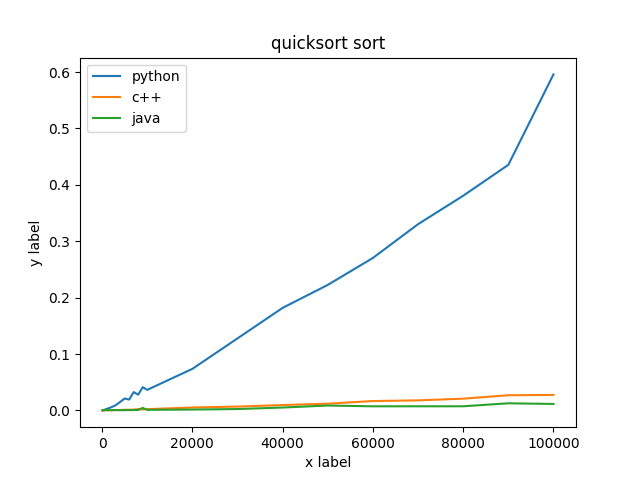
\includegraphics[scale=0.35]{img/quicksort_diagram.png}
                        \caption{QuickSort - Tiempo de ejecución}
                        \label{fig:quicksort_diagram}
                    \end{figure}
		        \end{itemize}
		    \end{frame}

		%%%% SELECTION SORT
		\subsection{Selection Sort}
		    \begin{frame}{Selection Sort - Definición}
    		    \begin{algorithm}[H]
                    \begin{algorithmic}[1]
                        \FOR{$i \gets 0$ to $N-1$}
                            \STATE $minIdx \gets i$
                            \FOR{$j \gets i+1$ to $N$}
                                \IF{$A[j] < A[minIdx]$}
                                    \STATE $minIdx \gets j$ 
                                \ENDIF
                            \ENDFOR
                            \STATE $A[j + 1] \gets key$
                        \ENDFOR
                    \end{algorithmic}
                    \caption{SELECTION-SORT(A)}
                    \label{alg:selection-sort}
                \end{algorithm}
    		\end{frame}
    		
    		\begin{frame}{Selection Sort - Análisis}
    		     \begin{itemize}
    		         \item Ordena un Array por encontrar repetidamente el mínimo elemento, en orden ascendente, desde la parte desordenada y poniéndolo al inicio. El algoritmo mantiene un array ya ordenado y otro desordenado.
    		         \item El algoritmo tiene un costo de $O(n^2)$ \cite{Heineman2008}
    		         
    		         \begin{figure}[H]
        				\centering
        				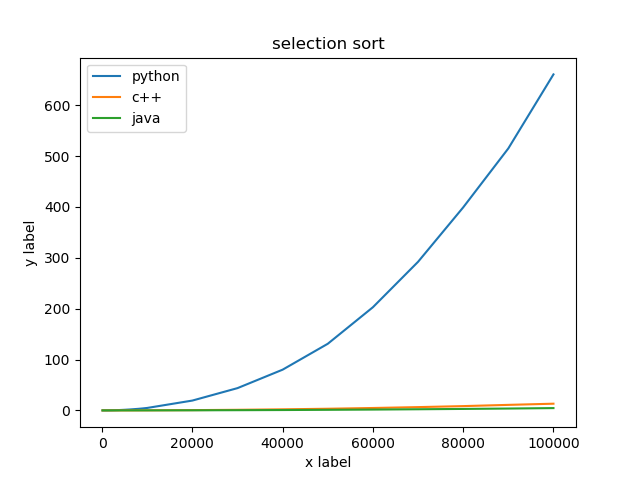
\includegraphics[scale=0.35]{img/selection_diagram.png}
        				\caption{Tiempo de Ejecución Selection Sort}
        				\label{fig: selection_sort_fig1}
        			\end{figure}
    		         
    		     \end{itemize}
    		    
    		\end{frame}
	
		
	%%%% COMPARACION
	\section{Comparación del tiempo de Procesamiento}
		\begin{frame}{Resultado en C++}
			\justifying
			\begin{figure}[H]
        				\centering
        				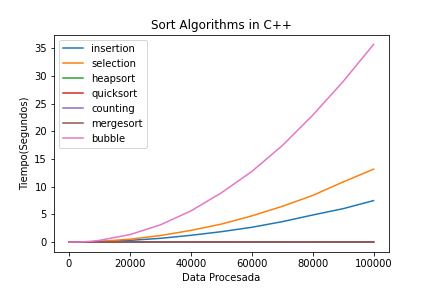
\includegraphics[scale=0.5]{img/sort-algorithms-cpp.png}
        				\caption{Algoritmos de Ordenamiento en C++}
        				\label{fig:sort-algorithms-cpp}
        			\end{figure}
		\end{frame}
		\begin{frame}{Resultado en Python}
			\justifying
			\begin{figure}[H]
        				\centering
        				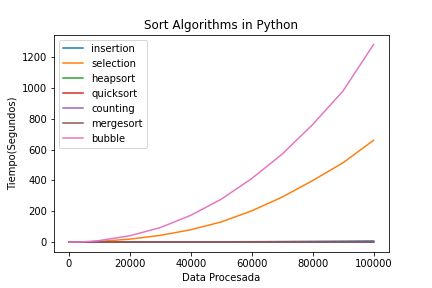
\includegraphics[scale=0.5]{img/sort-algorithms-python.png}
        				\caption{Algoritmos de Ordenamiento en Python}
        				\label{fig:sort-algorithms-python}
        			\end{figure}
		\end{frame}
		\begin{frame}{}
		    \centering
		    
		    {
		        \Large
		        GRACIAS
		    }
		    
		    \begin{figure}[H]
				\centering
				
\includegraphics[scale=0.5]{img/qr_repositorio.png}
				
				\label{fig:qr_repositorio}
			\end{figure}
			
			Repositorio: \url{https://github.com/jabarcamu/EDA_Practica1}
		    
		\end{frame}

%\appendix
\section{Referencias}
%\subsection<presentation>*{Referencias}

% All of the following is optional and typically not needed. 
%\appendix


\begin{frame}[t, allowframebreaks]
    \frametitle{References}
    \bibliographystyle{ieeetr}
    \bibliography{biblio}
\end{frame}



\end{document}